\documentclass[11pt]{article}
\usepackage[utf8]{inputenc}
\usepackage[T1]{fontenc}
\usepackage[margin=1in]{geometry}
\usepackage{amsmath,amssymb,booktabs,array,tabularx,ragged2e}
\usepackage{graphicx}
\usepackage{tikz}
\usetikzlibrary{arrows.meta,fit}
\usepackage[strings]{underscore}
\newcolumntype{Y}{>{\RaggedRight\arraybackslash}X}

\title{Asymmetric Attention Heads: Hierarchical Group-Level Control for Quality-Constrained Attention Compute Efficiency}
\author{Zimu Zhao}
\date{}

\begin{document}
\maketitle

\begin{abstract}
  Standard multi-head attention (MHA) allocates attention computation uniformly across heads, even though heads often differ in specialization and execution utility. This work studies whether structured, unequal allocation across heads can reduce effective attention computation while preserving model quality. \textbf{AAH} stands for \textbf{Asymmetric Attention Heads}: \emph{Asymmetric} indicates uneven computation across heads or head groups, \emph{Attention} indicates a change to how MHA is executed, and \emph{Heads} indicates that control is applied across heads within the standard multi-head structure. We present \textbf{AAH-v3}, an execution-aware extension of MHA whose key controller mechanism is wide joint sibling scoring over enriched head-group representations. AAH-v3 builds EMA-smoothed head features, separates level-0 grouping from upper-level hierarchy construction, constrains discrete window decisions top-down, maps level-0 decisions back to heads, and executes grouped causal local attention. The current evidence emphasizes a specific regime conclusion: wide joint scoring is the first viable non-degenerate grouped controller; at the main 1B / 512-token / 1000-step budget, both learned regimes beat \texttt{grouping\_off}, shallow learned \([2]\) topology is sufficient, and deeper \([2,2,2,2]\) hierarchy is not clearly necessary there. AAH-v3 preserves the Transformer block interface and flat output merge while changing the MHA execution policy. We frame the contribution as a quality-constrained efficiency study in compute-proxy space, with wall-clock throughput treated as a secondary systems outcome because runtime depends on masking behavior, kernels, and hardware.
\end{abstract}

\clearpage
\begin{figure}[p]
  \centering
  \resizebox{\textwidth}{!}{%
    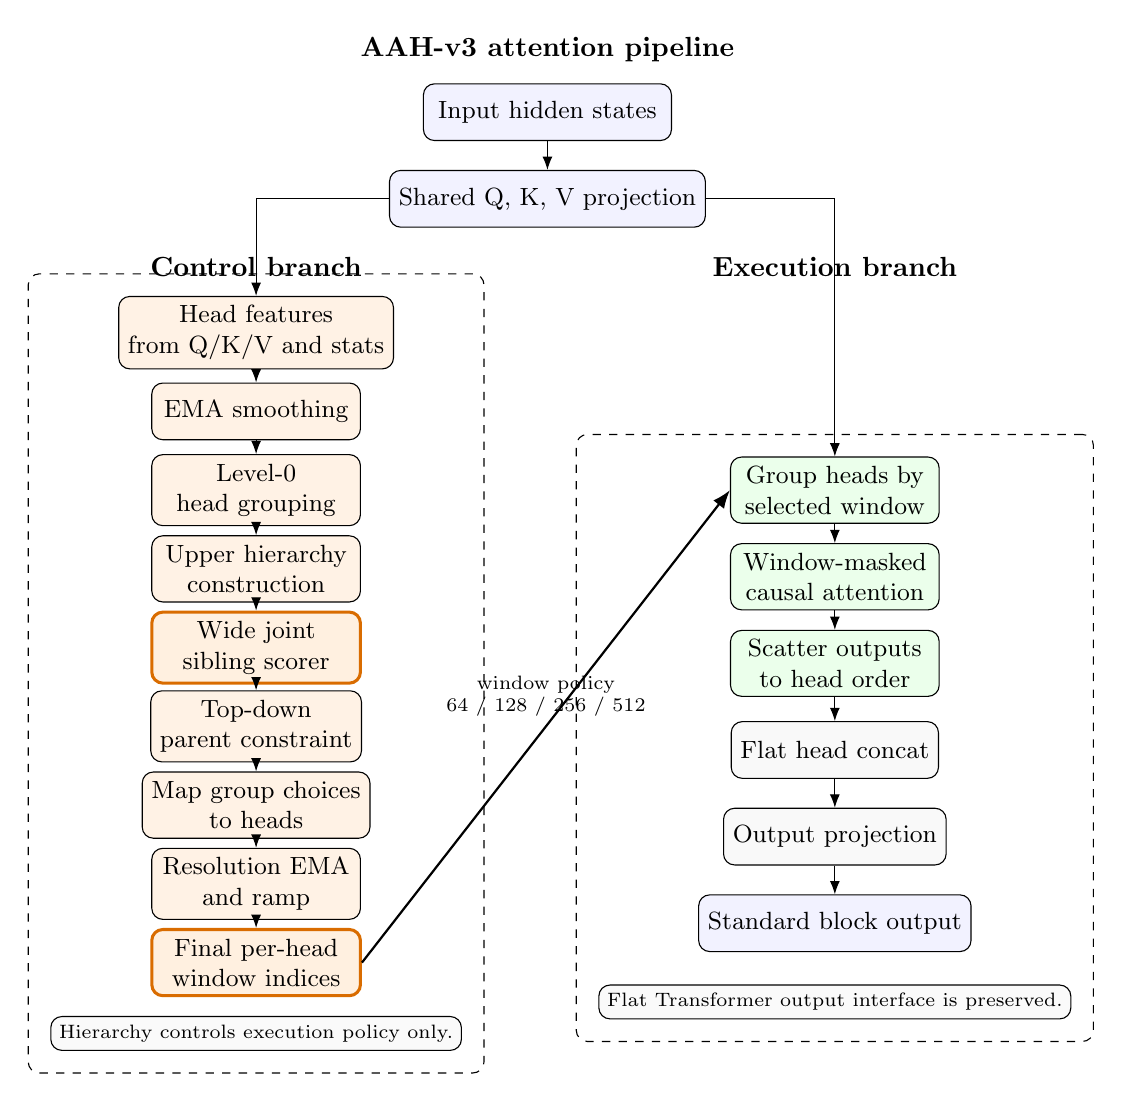
\begin{tikzpicture}[
        font=\small,
        >=Latex,
        block/.style={draw, rounded corners, align=center, minimum width=2.55cm, minimum height=0.72cm, fill=gray!5},
        control/.style={draw, rounded corners, align=center, minimum width=2.65cm, minimum height=0.72cm, fill=orange!10},
        exec/.style={draw, rounded corners, align=center, minimum width=2.65cm, minimum height=0.72cm, fill=green!8},
        policy/.style={draw=orange!85!black, line width=1.1pt, rounded corners, align=center, minimum width=2.65cm, minimum height=0.72cm, fill=orange!12},
        shared/.style={draw, rounded corners, align=center, minimum width=3.15cm, minimum height=0.72cm, fill=blue!5},
        note/.style={align=center},
        annot/.style={draw, rounded corners, align=center, font=\scriptsize, inner sep=3pt, fill=gray!4},
        panel/.style={draw, rounded corners, dashed, inner sep=0.28cm}
      ]
      \node[note, font=\bfseries] at (0,3.45) {AAH-v3 attention pipeline};

      \node[shared] (x) at (0,2.65) {Input hidden states};
      \node[shared] (qkv) at (0,1.55) {Shared Q, K, V projection};

      \node[note, font=\bfseries] at (-3.7,0.68) {Control branch};
      \node[control] (feat) at (-3.7,-0.15) {Head features\\from Q/K/V and stats};
      \node[control] (ema) at (-3.7,-1.15) {EMA smoothing};
      \node[control] (g0) at (-3.7,-2.15) {Level-0\\head grouping};
      \node[control] (hier) at (-3.7,-3.15) {Upper hierarchy\\construction};
      \node[policy] (score) at (-3.7,-4.15) {Wide joint\\sibling scorer};
      \node[control] (parent) at (-3.7,-5.15) {Top-down\\parent constraint};
      \node[control] (map) at (-3.7,-6.15) {Map group choices\\to heads};
      \node[control] (ramp) at (-3.7,-7.15) {Resolution EMA\\and ramp};
      \node[policy] (win) at (-3.7,-8.15) {Final per-head\\window indices};

      \node[note, font=\bfseries] at (3.65,0.68) {Execution branch};
      \node[exec] (bucket) at (3.65,-2.15) {Group heads by\\selected window};
      \node[exec] (local) at (3.65,-3.25) {Window-masked\\causal attention};
      \node[exec] (scatter) at (3.65,-4.35) {Scatter outputs\\to head order};
      \node[block] (concat) at (3.65,-5.45) {Flat head concat};
      \node[block] (proj) at (3.65,-6.55) {Output projection};
      \node[shared] (out) at (3.65,-7.65) {Standard block output};

      \draw[->] (x) -- (qkv);
      \draw[->] (qkv) -| (feat);
      \draw[->] (feat) -- (ema);
      \draw[->] (ema) -- (g0);
      \draw[->] (g0) -- (hier);
      \draw[->] (hier) -- (score);
      \draw[->] (score) -- (parent);
      \draw[->] (parent) -- (map);
      \draw[->] (map) -- (ramp);
      \draw[->] (ramp) -- (win);

      \draw[->] (qkv) -| (bucket);
      \draw[->] (bucket) -- (local);
      \draw[->] (local) -- (scatter);
      \draw[->] (scatter) -- (concat);
      \draw[->] (concat) -- (proj);
      \draw[->] (proj) -- (out);
      \draw[->, thick] (win.east) -- node[above, font=\scriptsize, align=center] {window policy\\64 / 128 / 256 / 512} (bucket.west);

      \node[annot] (note-control) at (-3.7,-9.05) {Hierarchy controls execution policy only.};
      \node[annot] (note-exec) at (3.65,-8.65) {Flat Transformer output interface is preserved.};

      \node[panel, fit=(feat) (ema) (g0) (hier) (score) (parent) (map) (ramp) (win) (note-control)] {};
      \node[panel, fit=(bucket) (local) (scatter) (concat) (proj) (out) (note-exec)] {};
    \end{tikzpicture}%
  }
  \caption{AAH-v3 attention pipeline. The same Q/K/V tensors feed a control branch and an execution branch. The control branch builds EMA-smoothed head features, constructs level-0 groups and upper hierarchy, applies wide joint sibling scoring, enforces top-down parent constraints, and maps the resulting window decisions back to heads. The execution branch groups heads by selected window, applies window-masked causal attention, and returns to the standard flat multi-head output interface.}
  \label{fig:aah_v3_overview}
\end{figure}
\clearpage

\section{Introduction}

Transformers rely on multi-head attention (MHA), where each head is typically executed with a uniform attention pattern and full attended span. This design is simple and robust, but it may over-allocate computation: not all heads require the same attended region to make useful contributions at every stage of execution. This motivates a central question: \textbf{can attention computation be reduced through structured, unequal head allocation while maintaining model quality?}

We study this question through the \textbf{Asymmetric Attention Heads (AAH)} line of methods, with \textbf{AAH-v3} as the final method analyzed here. AAH-v3 controls MHA execution across heads and head groups by selecting discrete causal attention windows, while preserving the standard Transformer block interface and flat output merge. The method changes the \textbf{MHA execution policy across heads}, rather than the output topology of the Transformer block.

Our evaluation scope is intentionally constrained. We treat \textbf{effective attention computation} as the primary optimization target, measured by \textbf{Attention Compute Ratio (ACR)} and aligned FLOPs-style proxies, and treat validation quality as the primary guardrail. Runtime metrics such as inference tokens per second are reported only as secondary systems outcomes, because reductions in compute proxy do not guarantee proportional wall-clock gains across different masking implementations, kernels, and hardware platforms.

Earlier internal variants explored static and preliminary dynamic asymmetry, but are not part of the main paper narrative. \textbf{AAH is the sole main method studied in this paper.} We study uneven head-level compute allocation within the standard Transformer interface and evaluate AAH primarily through quality-constrained compute-proxy efficiency, with runtime treated as secondary.

Our contributions are as follows:
\begin{enumerate}
  \item \textbf{Method.} We present AAH-v3 as an MHA-level, cross-head execution controller using EMA-smoothed head features, mixed hierarchy construction, enriched controller inputs, wide joint sibling scoring, top-down parent constraints, and grouped causal local attention.
  \item \textbf{Controller finding.} We identify wide joint sibling scoring as the first viable non-degenerate grouped controller in this line: sibling-paired groups are scored jointly, and the joint scorer replaces paired sibling logits rather than adding a bias.
  \item \textbf{Regime comparison.} We compare pure baseline, \texttt{grouping\_off}, shallow \texttt{freeze\_learned\_topology}, and deep practical reuse. At the current 1B, sequence-length 512, 1000-step, three-seed budget, both learned regimes beat \texttt{grouping\_off}; shallow learned \([2]\) is sufficient, and deep \([2,2,2,2]\) is not clearly necessary.
  \item \textbf{Claim boundaries.} We do not claim that deep hierarchy is generally necessary, that full continuous adaptivity is best, or that the method is already long-context-ready; sequence length 1024 remains a stress test and open limitation.
\end{enumerate}

\section{Motivation and Problem Diagnosis}

\subsection{Uniform head execution as potential over-allocation}

Standard MHA assigns comparable attention computation to all heads in a layer. This is robust, but it can over-allocate computation when heads differ in specialization, redundancy, and context-dependent utility. In that case, equal-width execution across all heads is stronger than necessary.

AAH targets this diagnosis directly: head-level computation should be allocated unevenly while preserving standard Transformer block semantics. The goal is therefore not generic sparsification, but \emph{quality-constrained compute redistribution within the multi-head interface}.

\subsection{Why AAH is needed}

Early static asymmetry confirms that unequal allocation is possible, but static policies are too rigid across context and training phases. Preliminary dynamic asymmetry improves flexibility but is sensitive to instability and control noise.

AAH-v3 addresses this by using grouped dynamic control with enriched hierarchy-aware features, joint sibling scoring, and constrained resolution decisions. This design keeps the external Transformer interface unchanged while providing a stable MHA-level execution policy across heads.

\subsection{Proxy efficiency versus systems efficiency}

A second diagnosis is methodological: reduced effective attended region does not guarantee proportional wall-clock speedup. Masking path, kernel behavior, and hardware characteristics can decouple algorithmic proxy gains from throughput. For this reason, AAH is evaluated primarily through \textbf{compute proxies under quality constraints}, while runtime is analyzed as a secondary systems result.

\section{Related Work}

\subsection{Standard MHA and head redundancy}

Standard MHA allocates comparable execution patterns and attention span across all heads in a layer. However, many empirical analyses of Transformers suggest that heads are not equally useful, equally specialized, or equally necessary at all times. This motivates studying whether head-level compute can be allocated unevenly while preserving the standard Transformer block contract.

\subsection{Sparse, local, and approximate attention}

A large body of work reduces attention cost through sparsity, locality, approximation, retrieval, indexing, and linear-attention formulations. AAH is positioned differently. It is \textbf{not} a sparse-attention replacement, \textbf{not} a linear-attention reformulation, and \textbf{not} a topology-changing output design. Instead, AAH provides \textbf{head-level execution control within standard Transformer block semantics}. Unlike grouped-query attention (GQA) or multi-query attention (MQA), which reduce or share K/V heads, AAH-v3 keeps the full attention-head set and adapts compute by assigning different causal local window spans to heads or head groups.

\subsection{Systems-aware efficiency and runtime}

Algorithmic compute reduction and wall-clock speed are not equivalent. AAH is also \textbf{not} a kernel-optimization method: it does not by itself guarantee kernel-level FLOPs or throughput gains. We therefore evaluate AAH primarily through compute proxies under quality constraints, and treat runtime as a secondary systems outcome.

\section{Background: Standard Multi-Head Attention}

Let \(X \in \mathbb{R}^{L \times d}\) denote the input sequence representation, where \(L\) is sequence length and \(d\) is model dimension. For each head \(h \in \{1,\dots,H\}\),
\[
  Q_h = XW_h^Q,\qquad K_h = XW_h^K,\qquad V_h = XW_h^V.
\]

The head output is
\[
  O_h = \operatorname{softmax}\!\left(\frac{Q_hK_h^\top}{\sqrt{d_h}} + M\right)V_h,
\]
where \(d_h\) is the head dimension and \(M\) is the causal mask. The final multi-head attention output is
\[
  O = \operatorname{Concat}(O_1,\dots,O_H)W^O.
\]

This formulation has two important properties. First, all heads operate in parallel on the same layer input. Second, all heads use the same full-width attention pattern over the sequence. In other words, standard MHA allocates \textbf{uniform attention computation across heads}.

If each head attends over the full causal context, the dominant attention-score computation scales proportionally to
\[
  \sum_{h=1}^{H} L^2 d_h,
\]
ignoring constant factors and non-attention terms. This quadratic dependence on sequence length makes attention a natural target for execution-aware compute reduction.

\subsection*{Notation}

\begin{center}
  \begin{tabularx}{\textwidth}{>{\bfseries}l Y}
    \toprule
    Symbol & Meaning \\
    \midrule
    \(L\) & sequence length \\
    \(d\) & model dimension \\
    \(d_h\) & head dimension \\
    \(H\) & number of heads \\
    \(N\) & number of layers \\
    \(\mathcal H_g\) & set of heads in group \(g\) \\
    \(\pi(h)\) & head-to-group mapping \\
    \(\psi_h\) & per-head feature vector \\
    \(\phi_g\) & aggregated group feature vector \\
    \(c_g\) & group control decision / selected window index \\
    \(\mathcal W\) & discrete window set \\
    \(L_{k,h}\) & selected attention width for head \(h\) \\
    \(\tilde L_{k,h}\) & clamped effective key width for head \(h\) \\
    \(\mathrm{ACR}\) & Attention Compute Ratio \\
    \(M\) & causal mask \\
    \(Q_h,K_h,V_h\) & head projections \\
    \bottomrule
  \end{tabularx}
\end{center}

\section{Method: AAH-v3}

\subsection{Method overview}

AAH-v3 augments standard multi-head attention with hierarchical execution control over heads and head groups. It preserves the Transformer block contract: the model still forms \(Q/K/V\) projections, computes scaled dot-product attention under a causal mask, concatenates head outputs, and applies the usual output projection. The change is the MHA execution policy: different heads may use different causal local windows selected by a hierarchy-aware controller.

Conceptually, AAH-v3 builds a hierarchy-aware representation of head groups and then solves a constrained discrete decision problem over attention windows. The representation side summarizes current \(Q/K/V\) behavior and recent attention diagnostics, smooths these signals over time, forms level-0 head groups, and aggregates them into upper-level groups. The decision side enriches each group representation with level, parent, global, and size information, then selects window indices that are consistent with the hierarchy.

The central controller shift from earlier drafts is the move from independent group scoring to \textbf{joint sibling scoring}. Rather than asking each group to choose a window in isolation, AAH-v3 scores sibling groups together using enriched representations and directional differences. This makes the sibling contrast part of the decision problem itself; the resulting logits replace the paired siblings' independent logits, and the selected discrete windows are propagated top-down before head-level execution.

This organization also separates four objects that are easy to conflate: level-0 head grouping, upper-level hierarchy construction, hierarchy-aware decision scoring, and the final execution mapping from group decisions to per-head windows.

\subsection{Head features and EMA smoothing}

For each head, AAH-v3 forms a \emph{base} feature from current \(Q/K/V\) statistics and previous attention diagnostics. In generic form,
\[
  g = [|\bar q|,\ \sigma(q),\ |\bar k|,\ \sigma(k),\ |\bar v|,\ \sigma(v),\ \text{entropy},\ \text{norm},\ \text{usage}].
\]
For head \(h\), this gives the per-head feature
\[
  x_h = [|\bar q_h|,\ \sigma(q_h),\ |\bar k_h|,\ \sigma(k_h),\ |\bar v_h|,\ \sigma(v_h),\ e_h,\ n_h,\ u_h].
\]
The first six entries summarize current projection behavior from the current raw \(Q/K/V\) pass. The final three entries \((e_h,n_h,u_h)\) are previous attention diagnostics: entropy, output norm, and usage from the most recent stored attention statistics.

This base feature \(x_h\) is not yet the controller input. It is first smoothed and aggregated into group features; later, Section~5.4 enriches those group features with hierarchy-level, parent, global, and size information.

Head features are temporally smoothed before hierarchy construction:
\[
  \bar x_{h,t} = \alpha \bar x_{h,t-1} + (1-\alpha)x_{h,t}.
\]
In the final 512-token configurations, control updates occur every five steps and the feature EMA coefficient is \(\alpha=0.9\). Between control updates, the cached per-head window indices are reused.

\subsection{Hierarchy construction}

AAH-v3 deliberately separates \textbf{level-0 head grouping} from \textbf{upper-level group hierarchy}. This is a major correction relative to older draft wording: the hierarchy does \emph{not} use one global similarity rule.

\textbf{Level 0: cosine head grouping with fallback.} The bottom level clusters EMA-smoothed head features using cosine-based centroid-threshold clustering. If this clustering collapses to a single group, AAH-v3 applies a deterministic forced-bipartition fallback. This fallback is not random and not PCA-based: it selects the least-similar anchor pair, then assigns the remaining heads according to their relative similarity to the two anchors. The fallback is a robustness mechanism that ensures a nontrivial level-0 partition; it is not the main contribution.

\textbf{Upper levels: \texttt{cosine\_normdiff} group hierarchy.} Upper levels are built over aggregated group features using cosine similarity penalized by relative norm difference:
\[
  \operatorname{sim}(i,j) = \cos(x_i,x_j) - \lambda \cdot \frac{\left|\lVert x_i\rVert - \lVert x_j\rVert\right|}{\max(\lVert x_i\rVert,\lVert x_j\rVert,\epsilon)}.
\]
The final configurations use \(\lambda=16.0\) and \(\epsilon=10^{-6}\). Thus, level 0 uses cosine clustering with forced bipartition allowed, while upper levels use the modified norm-aware similarity. This distinction should be read as part of the method definition, not as an incidental implementation detail.

For a hierarchy with \(L\) levels, the normalized level coordinate is
\[
  r_\ell = \frac{\ell}{\max(1, L-1)}.
\]
The current evidence does not make deeper hierarchy the main success story. At the main 512-token budget, shallow learned \([2]\) is competitive or slightly better than deep practical \([2,2,2,2]\), so deeper hierarchy is not currently the main winning factor.

\subsection{Enriched controller inputs}

The controller operates on enriched group representations, not raw pooled group features. For item \(i\) at hierarchy level \(\ell\), the enriched input is
\[
  u_i^{(\ell)} = [g_i^{(\ell)},\ r_\ell,\ g_i^{(\ell)} - p_i^{(\ell)},\ g_i^{(\ell)} - \bar g^{(\ell)},\ s_i^{(\ell)}].
\]
Here \(g_i^{(\ell)}\) is the base group feature at level \(\ell\), obtained by aggregating lower-level features according to the hierarchy. The scalar \(r_\ell\) identifies the normalized hierarchy level. The parent feature \(p_i^{(\ell)}\) is the feature of item \(i\)'s parent when a parent exists, giving the parent-difference term \(g_i^{(\ell)}-p_i^{(\ell)}\). The global mean \(\bar g^{(\ell)}\) is the mean feature over items at the same level, giving the level-wise offset \(g_i^{(\ell)}-\bar g^{(\ell)}\). Finally, \(s_i^{(\ell)}\) records the group-size fraction.

With the 9-dimensional base feature, enriched mode has dimension \(9+1+9+9+1=29\). This enriched representation is the input to both the base controller logits and the joint sibling scorer.

\subsection{Joint sibling scoring}

Joint sibling scoring is the final AAH-v3 controller design and the main controller change relative to earlier independent-scoring variants. Under independent scoring, sibling groups are evaluated separately, as shown in Figure~\ref{fig:joint_sibling_scoring}(a). When sibling features are very similar, a shared scorer can produce nearly identical rankings over candidate windows even when different assignments would be preferable. AAH-v3 addresses this by scoring the ordered sibling pair jointly, making the contrast between siblings part of the decision, as shown in Figure~\ref{fig:joint_sibling_scoring}(b).

\begin{figure}[!htbp]
  \centering
  \resizebox{\textwidth}{!}{%
    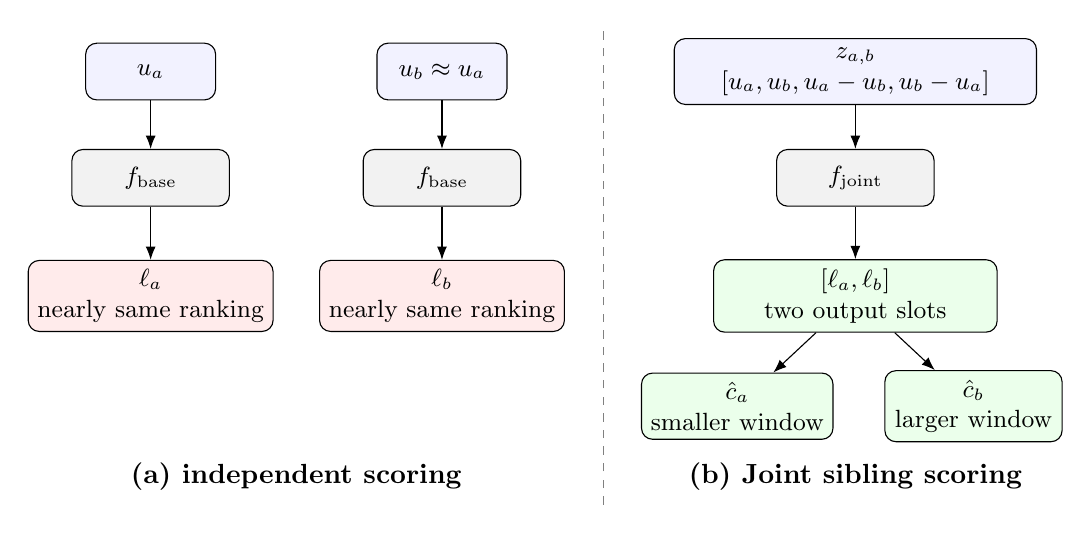
\begin{tikzpicture}[
        font=\small,
        >=Latex,
        box/.style={draw, rounded corners, align=center, minimum width=1.65cm, minimum height=0.72cm, fill=blue!5},
        scorer/.style={draw, rounded corners, align=center, minimum width=2.0cm, minimum height=0.72cm, fill=gray!10},
        bad/.style={draw, rounded corners, align=center, minimum width=2.25cm, minimum height=0.72cm, fill=red!8},
        good/.style={draw, rounded corners, align=center, minimum width=2.25cm, minimum height=0.72cm, fill=green!8},
        note/.style={align=center}
      ]
      \node[box] (ua) at (-5.65,2.0) {$u_a$};
      \node[box] (ub) at (-1.95,2.0) {$u_b \approx u_a$};
      \node[scorer] (fa) at (-5.65,0.65) {$f_{\mathrm{base}}$};
      \node[scorer] (fb) at (-1.95,0.65) {$f_{\mathrm{base}}$};
      \node[bad] (la) at (-5.65,-0.85) {$\ell_a$\\nearly same ranking};
      \node[bad] (lb) at (-1.95,-0.85) {$\ell_b$\\nearly same ranking};
      \node[note, font=\bfseries] at (-3.8,-3.15) {(a) independent scoring};

      \draw[->] (ua) -- (fa);
      \draw[->] (ub) -- (fb);
      \draw[->] (fa) -- (la);
      \draw[->] (fb) -- (lb);

      \draw[dashed, gray] (0.1,-3.5) -- (0.1,2.55);

      \node[box, minimum width=4.6cm] (pair) at (3.3,2.0) {$z_{a,b}$\\$[u_a,u_b,u_a-u_b,u_b-u_a]$};
      \node[scorer] (fjoint) at (3.3,0.65) {$f_{\mathrm{joint}}$};
      \node[good, minimum width=3.6cm] (jointlogits) at (3.3,-0.85) {$[\ell_a,\ell_b]$\\two output slots};
      \node[good] (ca) at (1.8,-2.25) {$\hat c_a$\\smaller window};
      \node[good] (cb) at (4.8,-2.25) {$\hat c_b$\\larger window};
      \node[note, font=\bfseries] at (3.3,-3.15) {(b) Joint sibling scoring};

      \draw[->] (pair) -- (fjoint);
      \draw[->] (fjoint) -- (jointlogits);
      \draw[->] (jointlogits) -- (ca);
      \draw[->] (jointlogits) -- (cb);
    \end{tikzpicture}%
  }
  \caption{Independent sibling scoring versus joint sibling scoring. Panel (a) shows sibling groups scored separately by the base scorer. Panel (b) shows the ordered sibling pair scored jointly, producing two output-logit slots for the two siblings.}
  \label{fig:joint_sibling_scoring}
\end{figure}

For a sibling pair \((a,b)\), AAH-v3 builds the order-sensitive input
\[
  z_{a,b} = [u_a,\ u_b,\ u_a-u_b,\ u_b-u_a].
\]
This representation is not symmetric under swapping \(a\) and \(b\): the first output slot corresponds to the first sibling and the second output slot corresponds to the second sibling. Because the scorer observes both \(u_a-u_b\) and \(u_b-u_a\), it can assign different logits and complementary windows to siblings with otherwise similar base features.

The wide joint sibling scorer outputs two logit vectors at once:
\[
  [\ell_a,\ell_b] = \operatorname{reshape}(f_{\text{joint}}(z_{a,b}), 2, K),
\]
where \(K=|\mathcal W|\). In the final method, \(\mathcal W=[64,128,256,512]\) for 512-token runs. The sibling-specific raw choices are then
\[
  \hat c_a^{(\ell)}=\arg\max_k \ell_{a,k}^{(\ell)}, \qquad
  \hat c_b^{(\ell)}=\arg\max_k \ell_{b,k}^{(\ell)}.
\]
For paired siblings, these joint logits replace the corresponding independently computed logits rather than acting as an additive correction or residual bias. Equivalently, the base controller may produce logits first, but the joint sibling scorer overwrites those logits for paired siblings before the argmax window decision.

\subsection{Window selection and parent index constraint}

For non-paired items, or after paired logits have been replaced, the same raw-choice rule can be written generically as
\[
  \hat c_i^{(\ell)} = \arg\max_k \ell_{i,k}^{(\ell)}.
\]
This raw choice is distinct from the parent-constrained choice. The candidate window list is ordered by increasing span, for example \(\mathcal W=[64,128,256,512]\). Thus, larger indices correspond to physically larger causal local windows. At the top level of the hierarchy, the raw choice is used directly; lower levels apply a parent index constraint:
\[
  c_i^{(\ell)} = \min(\hat c_i^{(\ell)},\ c_{\operatorname{parent}(i)}^{(\ell+1)}).
\]
This operation is an index-level top-down constraint, not the later execution-window bounding operation. Because \(\mathcal W\) is ordered by increasing span, the minimum operation has a direct physical meaning. A child group cannot select a larger attention-window span than its parent group. It does not force the child to copy the parent; a child can still choose a smaller window than its parent.

\subsection{Head mapping and execution}

After parent-constrained level-0 decisions are available, group decisions are mapped back to individual heads:
\[
  c_h = c_{g(h)}^{(0)}.
\]
This is the explicit bridge between hierarchy-level decisions and per-head MHA execution.

AAH-v3 smooths final per-head resolution indices before execution:
\[
  \tilde c_t = \operatorname{round}\left(\alpha \tilde c_{t-1} + (1-\alpha)c_t\right).
\]
This resolution EMA smooths the selected window index over time after hierarchy scoring and group-to-head mapping. It is not topology reuse, and it is not hierarchy smoothing: it acts only on the final per-head discrete resolution index. The final successful 512-token configurations include this smoothing with \(\alpha=0.15\).

Post-warmup ramping is a separate optional stabilization mechanism in the implementation. It is inactive in the current successful reported regime, so the active final path is no-ramp: hierarchy scoring, parent index constraint, group-to-head mapping, resolution EMA, execution-window mapping, and local attention.

The final execution window for head \(h\) is then mapped from the selected index and clamped to valid execution bounds:
\[
  W_h = \operatorname{clamp}(\mathcal W[c_h],\ W_{\min},\ T).
\]
For the main 512-token setting, \(W_{\min}=64\) and \(T=512\). This final execution-window clamp is distinct from the parent index constraint in Section~5.6.

Heads with the same selected window are grouped and executed together under causal local masking. For each selected window, the mask \(M_W\) allows only keys satisfying \(k\le q\) and \(k\ge q-W+1\). Attention is then
\[
  A = \operatorname{softmax}\left(\frac{QK^\top}{\sqrt d} + M_W\right), \quad Y = AV.
\]
A full-window choice \(W=T\) reduces to standard causal attention. In the current implementation, the strongest supported efficiency claim is reduction in effective attended region and compute-proxy metrics, not guaranteed kernel-level FLOPs or universal wall-clock speedup.

\subsection{What AAH-v3 changes relative to baseline}

Baseline MHA applies the same full causal attention pattern to all heads and then merges head outputs as usual:
\[
  O=\operatorname{Concat}(O_1,\dots,O_H)W^O.
\]
AAH-v3 keeps this output topology but changes the execution policy before the merge. Its real changes are learned head grouping, enriched controller inputs, wide joint sibling scoring, top-down constrained discrete window decisions, and grouped local causal execution. The wide joint sibling scorer is the key controller change: AAH-v3 is not an independent per-group scorer and not a mechanism operating inside a single attention head.
\section{Experimental Setup}

\subsection{Main regime}

The main validated regime is a 1B-parameter model trained at sequence length 512 for 1000 steps with three seeds. This is the regime where the current AAH-v3 method family is most mature and where the main claims are drawn. All comparisons use the same data pipeline, tokenizer, training budget, and evaluation protocol.

\subsection{Regimes compared}

The main result tables compare only the final method-family regimes:
\begin{itemize}
  \item \textbf{Pure baseline}: no AAH; standard Transformer MHA with ordinary causal attention.
  \item \textbf{\texttt{grouping\_off}}: the main learned-control baseline. It preserves the active AAH-v3 control-path comparison, but removes the learned grouping/topology advantage, so improvements over this row can be attributed to learned grouping and topology rather than wrapper infrastructure alone.
  \item \textbf{Shallow \texttt{freeze\_learned\_topology}}: the learned topology for the shallow \([2]\) configuration is established and then frozen. The topology is fixed, but group features, enriched controller inputs, joint sibling logits, parent-constrained decisions, and final head windows continue to be recomputed.
  \item \textbf{Deep practical reuse}: the cached level-0 head partition is reused after it is established. The level-0 topology is reused, but group features, upper hierarchy, parent maps, enriched inputs, joint sibling logits, parent-constrained decisions, and final head windows continue to be recomputed on control updates.
\end{itemize}

Additional regimes are treated as appendix or ablation material rather than central comparisons: \texttt{control\_off}, full adaptive, fixed random grouping, and freeze-after-warmup passthrough. These runs are useful for diagnosing mechanism behavior, but they should not be mixed into the main result table unless explicitly labeled as ablations.

These definitions distinguish topology reuse from decision freezing. In particular, \texttt{freeze\_learned\_topology} freezes learned topology, not the whole decision process; deep practical reuse freezes/reuses level-0 grouping, not group features or window choices.

\subsection{Evaluation protocol and metrics}

For the main 512-token regime, the headline comparison is:
\begin{center}
  \begin{tabularx}{\textwidth}{l l l Y}
    \toprule
    Model & Sequence length & Budget & Main compared methods \\
    \midrule
    1B & 512 & 1000 steps, 3 seeds & four main regimes listed in Section~6.2 \\
    \bottomrule
  \end{tabularx}
\end{center}

The interpretation priority is:
\begin{enumerate}
  \item quality: \texttt{val\_ppl}, then \texttt{val\_loss},
  \item compute proxy: \texttt{flops\_ratio} / ACR-style effective-attention ratios,
  \item runtime: \texttt{infer tok/s} as a secondary systems outcome,
  \item mechanism diagnostics: grouping stability, window distributions, sibling decisions, and parent-constraint statistics as supporting evidence.
\end{enumerate}
Runtime does not override quality-constrained compute-proxy conclusions, and mechanism diagnostics support interpretation rather than replacing quality metrics.

\subsection{Secondary long-context stress test}

A secondary stress test evaluates 1B models at sequence length 1024, comparing \texttt{grouping\_off}, shallow \texttt{freeze\_learned\_topology}, and deep practical reuse. This setting is a limitation-oriented transfer check, not the primary proof of the method. Current evidence should be framed conservatively: shallow remains better than deep in this stress test, but both learned-control regimes lose to \texttt{grouping\_off}. In this configuration, the learned-control settings are not long-context-ready.

\section{Main Results}

The current evidence supports a bounded result story. First, wide joint sibling scoring is the first viable non-degenerate grouped controller in this method line: paired siblings are scored jointly with directional differences and receive replacement logits. Second, learned grouping matters relative to \texttt{grouping\_off} in the main 512-token regime: both shallow \texttt{freeze\_learned\_topology} and deep practical reuse beat \texttt{grouping\_off} at the 1B / 512 / 1000-step setting. Third, shallow learned \([2]\) is sufficient at this budget; deep \([2,2,2,2]\) practical reuse is not clearly necessary.

The result should not be interpreted as showing that deep hierarchy is generally necessary, that full continuous adaptivity is the best regime, or that AAH-v3 is already solved for long-context use. The 1024-token experiment is therefore reported as a secondary stress test and limitation.

\begin{table}[ht]
  \centering
  \caption{Main comparison structure for the final AAH-v3 experiments. The main table is restricted to pure baseline, \texttt{grouping\_off}, shallow freeze, and deep practical reuse, and includes post-warmup throughput to expose the practical tradeoff. Numerical values should be filled only from the finalized result bundle.}
  \label{tab:main_regimes}
  \resizebox{\textwidth}{!}{%
    \begin{tabular}{lllccccl}
      \toprule
      Model & Seq. len. & Method & val\_ppl & val\_loss & flops\_ratio / ACR & post-warmup tok/s & Role \\
      \midrule
      1B & 512 & Pure baseline & TBD & TBD & 1.0000 & TBD & standard MHA reference \\
      1B & 512 & \texttt{grouping\_off} & TBD & TBD & TBD & TBD & learned-control baseline \\
      1B & 512 & Shallow \texttt{freeze\_learned\_topology} & TBD & TBD & TBD & TBD & main sufficient regime \\
      1B & 512 & Deep practical reuse & TBD & TBD & TBD & TBD & depth/reuse comparison \\
      \bottomrule
    \end{tabular}%
  }
\end{table}

\section{Long-Context Stress Test}

The 1B, sequence-length 1024 setting compares \texttt{grouping\_off}, shallow \texttt{freeze\_learned\_topology}, and deep practical reuse. Its role is to test whether the 512-token conclusions transfer under longer context. The current framing is deliberately negative/limited: shallow still beats deep, but both learned-control regimes lose to \texttt{grouping\_off}. Thus, long-context 1024 remains a stress case and the paper should not claim that AAH-v3 is already long-context-ready.

\begin{table}[ht]
  \centering
  \caption{Secondary long-context stress-test structure. This table is a limitation-oriented comparison, not the primary claim table. Current framing: shallow beats deep, but both lose to \texttt{grouping\_off}.}
  \label{tab:long_context}
  \resizebox{\textwidth}{!}{%
    \begin{tabular}{lllcccl}
      \toprule
      Model & Seq. len. & Method & val\_ppl & val\_loss & flops\_ratio / ACR & Interpretation \\
      \midrule
      1B & 1024 & \texttt{grouping\_off} & TBD & TBD & TBD & strongest stress-test reference \\
      1B & 1024 & Shallow \texttt{freeze\_learned\_topology} & TBD & TBD & TBD & better than deep, below \texttt{grouping\_off} \\
      1B & 1024 & Deep practical reuse & TBD & TBD & TBD & weaker learned-control stress result \\
      \bottomrule
    \end{tabular}%
  }
\end{table}

\section{Discussion and Limitations}

AAH-v3 demonstrates that MHA-level, cross-head execution control can be implemented without changing the Transformer block interface. The most important methodological change from earlier drafts is the final controller design: enriched controller inputs and wide joint sibling scoring replace the old independent-group-scoring narrative.

The evidence currently supports a conservative structural conclusion. Learned grouping matters relative to \texttt{grouping\_off} in the main 512-token regime, and shallow learned \([2]\) with frozen learned topology is sufficient at the main 1B / 512 / 1000-step / three-seed budget. This suggests that the main benefit comes from learning a useful grouping scaffold and applying the wide joint sibling controller, not necessarily from maintaining a deeper hierarchy throughout training. Deep practical reuse remains an important comparison, but the current budget does not establish that deep \([2,2,2,2]\) hierarchy is generally necessary.

The practical regimes are not all fully adaptive. Deep practical reuse reuses the level-0 head partition after it is cached, while continuing to recompute group features, upper hierarchy, parent maps, enriched inputs, joint scorer decisions, and final windows. Shallow \texttt{freeze\_learned\_topology} freezes learned topology, not the entire decision process. These distinctions are central to interpreting the experiments.

The long-context result is a stronger limitation than the 512-token result: at sequence length 1024, shallow remains better than deep, but both learned-control regimes lose to \texttt{grouping\_off}. This means the current evidence argues against presenting AAH-v3 as long-context-ready. Broader long-context training, stability diagnostics, and different hierarchy or controller choices remain future work.

Finally, ACR and \texttt{flops\_ratio} remain compute proxies. The current local-attention path controls effective attended region through masking and grouped execution, but runtime gains remain implementation-, kernel-, and hardware-dependent.

\section{Conclusion}

We presented AAH-v3, an implemented Asymmetric Attention Heads method for MHA-level execution control across heads. The final design uses EMA-smoothed head features, level-specific hierarchy construction, enriched controller inputs, wide joint sibling replacement scoring, top-down parent constraints, group-to-head window mapping, resolution EMA smoothing, and grouped causal local attention. The current leading candidate is shallow \texttt{freeze\_learned\_topology} at the main 1B / 512 / 1000-step / three-seed budget: it preserves the learned grouping scaffold without requiring a deeper maintained hierarchy. The main unresolved issue is long-context behavior, where the 1024-token stress test remains unfavorable for the learned-control regimes.
\appendix

\section{Appendix}

\subsection{Earlier Internal Variants}

\textbf{AAH-v1: static asymmetric heads.} This variant tested fixed asymmetric head roles such as static local-window or reduced-resolution assignments. It is retained only as historical context because static asymmetry did not reliably preserve quality.

\textbf{AAH-v2: preliminary dynamic control.} This variant introduced early dynamic resolution control, but stability and implementation issues prevented robust main-text use.

\textbf{AAH-v3: final method in this paper.} AAH-v3 is the sole main method. Appendix material should contain additional ablations, including full adaptive behavior, fixed-topology variants, controller-pairwise ablations, long-context diagnostics, and the finalized reproducibility bundle.

\end{document}
